\section{Benchmark NIST-9 "Wave Front"}
\label{sec:bench-9}

This is a standard benchmark for adaptive FEM algorithms. The exact solution is smooth but contains singular gradient in the re-entrant corner.
The equation solved is the Poisson's equation.

\begin{equation} \label{wave-front}
-\Delta u = f,
\end{equation}
in the domain $\Omega = (0, 1)^2$, equipped with Dirichlet boundary conditions
given by the exact solution.

The exact solution:
\begin{equation}\label{exact-nist-9}
u(x, y) = tan^{-1}(\alpha (r - r_{0})),
\end{equation}
where $r = \sqrt{(x - x_{loc})^{2} + (y - y_{loc})^{2}}$.
Here $(x_{loc}, y_{loc})$ is the center of the circular wave front,
$r_{0}$ is the distance from the wave front to the center of the circle,
and $\alpha$ gives the steepness of the wave front.
The right-hand side $f$ is calculated by inserting (\ref{exact-nist-9}) into (\ref{wave-front}).
The solution of NIST-9 with $\alpha = 50$, $(x_{loc}, y_{loc}) = (0.5, 0.5)$,
$r_{0} = 0.25$ is shown in Fig. \ref{fig:sln-nist09}.

\begin{figure}[!ht]
\centering
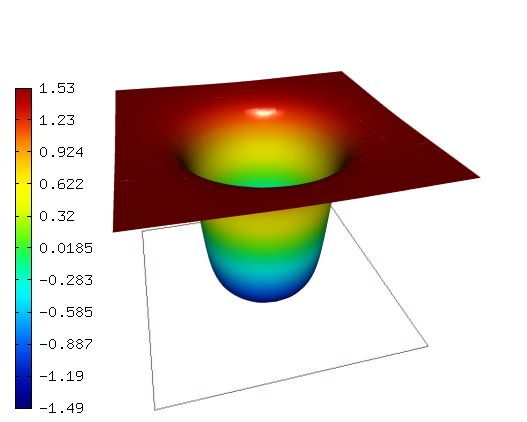
\includegraphics[height=6cm]{nist/nist-9/solution.png}
\caption{The solution to NIST-9 benchmark problem.}
\label{fig:sln-nist09}
\end{figure}
